\documentclass[12pt]{article}
\usepackage{geometry}
\geometry{a4paper}

\usepackage[parfill]{parskip}    % Activate to begin paragraphs with an empty line rather than an indent
\usepackage{graphicx}
\usepackage{amssymb}
\usepackage{epstopdf}
\usepackage{fancyhdr}
\usepackage{fullpage}
\usepackage{appendix}
\usepackage{newclude}
\usepackage{datetime}
\usepackage{hyperref}
\usepackage{color}
\usepackage{multicol}
\usepackage{tabularx}
\usepackage{enumerate}
\usepackage{enumitem}
\usepackage{listings}
\usepackage{wallpaper}
\usepackage{lastpage}
\usepackage{titling}
\usepackage{multind}
\usepackage[table]{xcolor}
\usepackage{mathtools}
\usepackage{tikz}
\usepackage{longtable}
\usepackage[section]{placeins}
%\geometry{landscape}
\usetikzlibrary{shapes,arrows}

\tikzstyle{block} = [rectangle, draw, text width = 6em, text centered, rounded corners, minimum height = 4em]
\tikzstyle{inputblock} = [rectangle, draw, text width = 24em, minimum height = 2.5em]
\tikzstyle{autographblock} = [rectangle, draw, fill = black!1, text height = 0, text depth = 2cm,text width = 24em, minimum height = 8em]
\tikzstyle{cloud} = [ellipse, draw, minimum height = 4em]
\tikzstyle{line} = [draw, -latex']

\makeindex{modules}


\newcommand{\usemodule}[1]{\index{modules}{#1}\texttt{#1}}

\definecolor{gray}{rgb}{0.5,0.5,0.5}
\definecolor{tableheader}{rgb}{0.7,0.7,0.7}

\setlist[description]{style=nextline}
\renewcommand{\familydefault}{\sfdefault}

% link setup
\hypersetup{
    colorlinks,
    citecolor=black,
    filecolor=black,
    linkcolor=black,
    urlcolor=black,
}

\DeclareGraphicsRule{.tif}{png}{.png}{`convert #1 `dirname #1`/`basename #1 .tif`.png}

% usefull commands:
\newcommand{\seeref}[1]{\ref{#1} p.\pageref{#1}}
%\newcommand{\see}[1]{ (zie \ref{#1} p.\pageref{#1})}
\newcommand{\seesee}[2]{ (zie \ref{#1} p.\pageref{#1},  \ref{#2} p.\pageref{#2})}

% style for code blocks
\lstset{
    linewidth=1\textwidth,
    breaklines=true,
    numbers=left,                   % where to put the line-numbers
    numberstyle=\tiny\color{gray},  % the style that is used for the line-numbers
    stepnumber=1,                   % the step between two line-numbers. If it's 1, each line 
    numbersep=5pt, 
    basicstyle=\footnotesize,
}

% Header and Footer settings
\URCornerWallPaper{0.13}{img/dop/koptekstlogo.png}
\pagestyle{fancy}
\fancyhead{}
\renewcommand{\headrulewidth}{0pt}

% Settings for table of contents.   
\setcounter{secnumdepth}{4}
\setcounter{tocdepth}{3}

\makeatletter
% some extra spacing for the table of contents
\renewcommand{\l@subsection}{\@dottedtocline{2}{1.5em}{3em}}
\renewcommand{\l@subsubsection}{\@dottedtocline{2}{2.7em}{4em}}

\renewcommand\paragraph{%
   \@startsection{paragraph}{4}{0mm}%
      {-\baselineskip}%
      {.5\baselineskip}%
      {\normalfont\normalsize\bfseries}}
\makeatother

\renewcommand{\dateseparator}{-}
\renewcommand{\figurename}{Figuur}

% Define variables
\newcommand{\customer}{Dimpact}
\newcommand{\projectname}{Dimpact}
\newcommand{\thecustomer}{\customer }
\newcommand{\customerdomain}{dimpact.nl}
\newcommand{\customerdomainfull}{http://www.dimpact.nl}
\newcommand{\customerdomainuc}{Dimpact.nl}
\newcommand{\authors}{David van Dijk \\ & Patrick Kraaij }
\newcommand{\version}{0.1}

\fancyfoot[L]{Functioneel ontwerp - \customer}
\fancyfoot[C]{v\version \ \ddmmyyyydate \today}
\fancyfoot[R]{\textbf{\thepage}\ / \pageref{LastPage}}

\title{\textbf{\customerdomainuc} \\ Functioneel Ontwerp}
\pretitle{\begin{flushleft}\LARGE}
\posttitle{\par\end{flushleft}}

\author{}  % skippen we voor maketitle
\date{}

% The actual Document:
\begin{document}
\ThisLRCornerWallPaper{0.8}{img/dop/voorbladlogo.png}

  \maketitle
 \vspace{-2.6cm}
  \begin{flushright}
\begin{tabularx}{4.6cm}{ X }
Dutch Open Projects         \\
Doornseweg 12                   \\  
3832 RL Leusden                 \\
T: +31[0]33 - 4 50 50 50        \\
F: +31[0]33 - 4 50 50 57        
\\*
\\*
\\*
\\*
\\*
\\*
\\*
\\*
\\*
\\*
\\*
\\*
\\*
\\*
\\*
\\*
\\*
\\*
\\*
\\*



\footnotesize
\copyright All rights reserved.         \\*
\footnotesize
No part of the contents of this publication may be reproduced, stored in a data processing system or transmitted in any form or by any means without the written permission of Dutch Open Projects B.V.

\end{tabularx}
\end{flushright}

\begin{tabularx}{\linewidth}{ p{3cm} X }
  Plaats & Leusden                                \\
  Laatst bijgewerkt & \ddmmyyyydate \today        \\
  Auteurs & \authors                          \\
  Versie & \version                                    \\
\end{tabularx}
\pagebreak




\pagebreak
\subsection*{Akkoord}
Voor akkoord:\\ \\
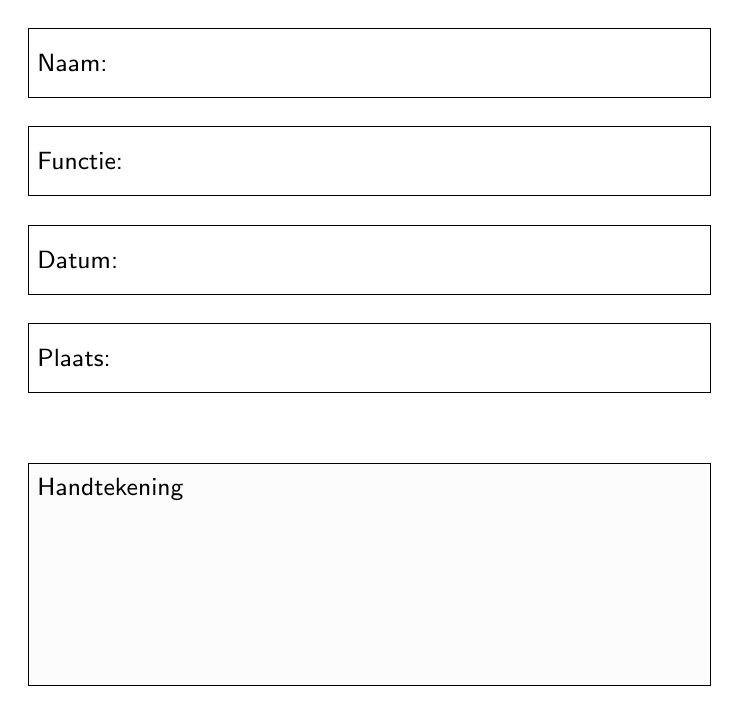
\begin{tikzpicture}
\tikzstyle{every node}=[font=\small];
\node [inputblock] (names) {Naam:};
\node [inputblock, below of = names, node distance = 1.25cm] (function) {Functie:};
\node [inputblock, below of = function, node distance = 1.25cm] (dates) {Datum:};
\node [inputblock, below of = dates, node distance = 1.25cm] (place) {Plaats:};
\node [autographblock, below of = place, node distance = 2.75cm] (autograph) {Handtekening};
\end{tikzpicture}
\pagebreak

% table of contents
\renewcommand*\contentsname{Inhoudsopgave}
\tableofcontents

\pagebreak


\section{Introductie}

\subsection{Management summary}
In dit document wordt de technische implementatie beschreven. Het is een blauwdruk voor ontwikkelaars. 

\subsection{Opbouw document}
Dit document dient als leidraad voor de bouw van dit project. Het belangrijkste onderdeel ervan zijn daarom de componenten. Deze zijn uitgesplitst naar componenten voor internet\seeone{internet} en intranet\seeone{intranet}.  Componenten bieden een opsplitsing van de functionaliteiten binnen de website, zowel zichtbaar als niet zichtbaar. Tijdens de bouw zal een ontwikkelaar aan \'{e}\'{e}n specifiek component tegelijk werken. Daarnaast worden in dit document een aantal randzaken zoals deployment\seeone{deployment} en performance\seeone{performance} en algemene eisen\seeone{algemeen} beschreven in eerdere hoofdstukken. In de appendix vindt met een overzicht van Drupal specifieke zaken zoals content types en views.
\subsection{Pagina's}\label{paginas}
In dit hoofdstuk worden een aantal pagina's beschreven zoals ontworpen in de wireframes.

\subsubsection{Pagina met inhoudsopgave}\label{paginainhoudsopgave}
Hier is geen speciaal content type voor, dit kan gedaan worden middels de aanwezige knoppen in de \emph{WYSIWYG}\seeone{wysiwyg} editor-balk. Hoe ankers aangemaakt kunnen worden staat beschreven in \emph{(Anker) links}\seeone{ankers}.

\subsubsection{Smoelenboek}\label{smoelenboek}
Het smoelenboek op het internet is een blok dat via Felix op een pagina gezet kan worden. In paragraaf \emph{Personenblok internet}\seeone{personenblokinternet} staat het te selecteren blok beschreven.



\section{Algemene componenten}
\label{sec:algemenecomponenten}

\subsection{Logo en naam}
\label{sec:logoennaam}
Op een beheerpagina in Drupal kan de naam van de website en het logo aangepast worden. Dit gaat door middel van een tekstveld in te vullen en een afbeelding te uploaden via een knop die ene bestand op de computer selecteert. Door op het logo of naam te klikken gaat de bezoeker naar de homepagina.

\subsection{Meta menu}
\label{sec:metamenu}
Het meta menu is een menu met links naar pagina's, dit menu heeft standaard de volgende items:
\begin{itemize}
  \item Home
  \item Sitemap
  \item Adressen en openingstijden
  \item Veelgestelde vragen
  \item RSS (Bij het klikken van deze link wordt de RSS getoond)
  \item Lees voor (Bij het klikken van deze link wordt Readspeaker geopend)
\end{itemize}
Dit menu is redactioneel uit te breiden.

\subsection{Tabs}
\label{sec:tabspagina}
De tabs is optioneel, deze functionaliteit kan in- en uitgeschakeld worden via een beheerpagina in Drupal door middel van een checkbox. %todo verder uitwerken

\subsection{Hoofdnavigatie}
\label{sec:hoofdnavigatie}
Het eerste niveau van het menu wordt getoond. Met een mouseover of een focus door middel van de tab-toets op het toetsenbord klapt het submenu van het betreffende hoofditem naar onderen open. Hier wordt onder elkaar het tweede niveau getoond. Bij het klikken of op de enter toets drukken ga je naar het betreffende pagina die aan het menu hangt.

\subsection{Zoekveld}
\label{sec:zoekveld}
Bij het zoekveld kan er gezocht worden door de website naar content op de website en content in documenten. Na het invullen van het zoekwoord kan er geklikt worden op de zoekbutton of op de entertoetst gedrukt worden, als de tekstcursor in het zoekveld staat, waarna de bezoeker naar het zoekresultatenpagina wordt geleidt. 

\subsection{Alfabetische balk}
\label{sec:alfabetischebalk}
De alfabetische balk is optioneel, deze functionaliteit kan in- en uitgeschakeld worden via een beheerpagina in Drupal door middel van een checkbox. Alle letters van het alfabet worden getoond, ook diegene die geen resultaat hebben. De functionaliteit verschilt hier; Javascript aan of Javascript uit in de browser.

\subsubsection{Javascript aan}
Bij het klikken op een letter verschijnt onder de balk een blok met daarin links naar pagina's die beginnen met de letter waarop gedrukt is. Als het blok is uitgeklapt en de bezoeker klik op een andere letter dan klapt het huidige blok weer in en verschijnt een andere blok met resultaten van de letter waarop is geklikt. De inhoud hiervan is redactioneel aan te passen. Er wordt geen uitzondering van gedrag gemaakt als de bezoeker twee keer op dezelfde letter klikt. Bij het klikken op het kruisje klapt het blok in.

\subsubsection{Javascript uit}
Bij het klikken op een letter wordt de bezoeker naar een pagina geleidt met redactioneel te bepalen content die begint met de letter waar de bezoeker op heeft geklikt.


\section{Blokken}
\label{sec:blokken}



\section{Overige functionaliteiten}
\label{sec:overigefunctionaliteiten}

\subsection{WYSIWYG}
We gebruiken een \emph{What You See Is What You Get} editor. DIt is een gebruiksvriendelijke manier van content invoeren in het CMS. De volgende opties zijn aanwezig:

\begin{itemize}
  \item Vet gedrukt
  \item Schuin
  \item Opsommings lijst
  \item Genummerde lijst 
  \item Definitie lijst
  \item Ongedaan maken
  \item Citaat
  \item Citaatblok
  \item Speciale tekens
  \item Kiezen uit opmaak
  \item Tabel
  \item Zoek en vervang
  \item Afkorting
  \item Acroniem
  \item Taal veranderen per woord
  \item Link invoegen
  \item Anker invoegen
  \item Media Invoegen
  \item Plakken speciaal
  \item Invoegen van woord
  \item Verwijderen van woord
\end{itemize}

\subsection{AddThis}

\subsection{Readspeaker}

\subsection{RSS}

\subsection{Sitemap}

\subsection{Responsive layout}


\end{document}
